\documentclass{article}
\title{Getting Started with LLGL}
\author{Lukas Hermanns}
\date{\today}

\usepackage{listings}
\usepackage{color}
\usepackage{pxfonts}
\usepackage{geometry}
\usepackage[T1]{fontenc}
\usepackage{xspace}
\usepackage{hyperref}
\usepackage{graphicx}
\usepackage{float}

\geometry{
	a4paper,
	left=15mm,
	right=15mm,
	top=20mm,
	bottom=20mm
}

\begin{document}

\definecolor{brightBlueColor}{rgb}{0.5, 0.5, 1.0}
\definecolor{darkBlueColor}{rgb}{0.0, 0.0, 0.5}

\def\LLGL{\textcolor{darkBlueColor}{LLGL}\xspace}

\lstset{
	language = C++,
	basicstyle = \footnotesize\ttfamily,
	commentstyle = \itshape\color{brightBlueColor},
	keywordstyle = \bfseries\color{darkBlueColor},
	stringstyle = \color{red},
	frame = single,
	tabsize = 4,
	showstringspaces=false,
	numbers=none
}

\maketitle


%----------------------------------------------------------------------------------------
%	INTRRODUCTION
%----------------------------------------------------------------------------------------

\section*{Introduction}

\LLGL (Low Level Graphics Library) is a thin abstraction layer for graphics APIs such as
OpenGL, Direct3D, and Vulkan. The library is written entirely in C++11, so you'll
need a modern C++ compiler, i.e. at least \textbf{VisualC++ 2013} for Windows,
\textbf{g++ 4.8} for Linux, or \textbf{Clang 3.1} for MacOS.


%----------------------------------------------------------------------------------------
%	BUILD PROCESS
%----------------------------------------------------------------------------------------

\section*{Build Process}

\subsection*{Dependencies}

\subsubsection*{GaussianLib}

The only required dependency is the header-only library
\href{https://github.com/LukasBanana/GaussianLib}{\textsc{GaussianLib}},
which is used for basic linear algebra computations with vectors and matrices.

\subsubsection*{OpenGL}

To build the OpenGL render system you need the OpenGL extension header files and an up-to-date graphics driver.
For Windows the header files \texttt{glext.h} and \texttt{wglext.h} are required.
For Linux the header files \texttt{glext.h} and \texttt{glxext.h} are required.
For MacOS no header files need to be downloaded, since the OpenGL version depends on the OS version.
You can find the header files at the \href{https://www.opengl.org/registry/#headers}{OpenGL registry page}.
Place the header files in the \texttt{include/GL/} folder of your compiler environment
or add the include path later in your build settings.

\subsubsection*{Direct3D}

Since VisualStudio 2013 the DirectX framework (of which Direct3D is a part of) is included within
the VisualStudio setup, so no further SDK needs to be installed.

\subsubsection*{Vulkan}

To build the Vulkan render system you need the \href{https://lunarg.com/vulkan-sdk/}{Vulkan SDK},
and of course a graphics driver which supports at least Vulkan 1.0.

\subsection*{Build Tool}

To build the \LLGL project files you need the build tool \href{https://cmake.org/}{CMake 2.8} or later.
The build process is now demonstrated with the CMake GUI on Windows, but it can also be configured
on a command line (more about this see \href{https://cmake.org/runningcmake/}{cmake.org/runningcmake}).

Set the source directory (``Where is the source code:'') to the \LLGL repository
and set the build directory (``Where to build the binaries'') where you want your project files.
In this example (see \ref{fig:cmake_mask1}) the source directory is \texttt{<\dots>/LLGL/repository}
and the build directory is \texttt{<\dots>/LLGL/build\_msvc14} because the project files are build
for MSVC14 (VisualStudio 2015).

Now set the \textsc{GaussianLib} include directory (in this example \texttt{<...>/GaussianLib/repository/include})
and click on ``Configure''. If everything worked quite well, you should see the message ``Configuring done''
in the lower box. To finally create the project files, clock on ``Generate''.
Then your project files should be located in the build directory you just set up previously.

\begin{figure}[H]
	\centering
	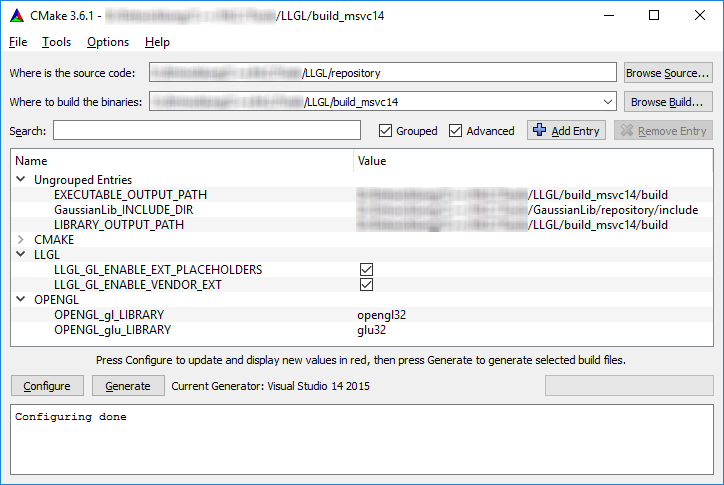
\includegraphics[width=0.9 \textwidth]{cmake_mask1}
	\caption{CMake GUI mask to set up the project files for VisualStudio 2015 (MSVC14).}
	\label{fig:cmake_mask1}
\end{figure}

There are a few options you can switch on and off, which will enable or disable the respective macro
when you compile the project:
\begin{itemize}
	\item \texttt{LLGL\_GL\_ENABLE\_EXT\_PLACEHOLDERS} \\
	Specifies whether OpenGL extensions should be replaced by placeholder procedures
	when they are not available. This may help debugging and should not influence the runtime performance.
	
	\item \texttt{LLGL\_GL\_ENABLE\_VENDOR\_EXT} \\
	Specifies whether vendor specific OpenGL extensions should be enabled or disabled.
	One of these extensions is for conservative rasterization
	(\texttt{GL\_NV\_conservative\_raster} and \texttt{GL\_INTEL\_conservative\_rasterization}) for instance.
	These extensions will only be loaded and used by the runtime if they are available on the host platform.
\end{itemize}


%----------------------------------------------------------------------------------------
%	API OVERVIEW
%----------------------------------------------------------------------------------------

\newpage

\section*{API Overview}

LLGL has a very simple and unified API design.

\begin{lstlisting}
class RenderSystem
{
	static shared_ptr<RenderSystem> Load(string moduleName);
}
\end{lstlisting}


%----------------------------------------------------------------------------------------
%	HELLO TRIANGLE
%----------------------------------------------------------------------------------------

\newpage

\section*{Hello Triangle}

After we have set up the library, we can start rendering some geometry.

\begin{lstlisting}
#include <LLGL/LLGL.h>
\end{lstlisting}


%----------------------------------------------------------------------------------------
%	APPENDIX
%----------------------------------------------------------------------------------------

\newpage

\section*{Appendix}

Foo bar ...






\end{document}
